
\section{Network}
\label{sec:network}

The basis network architecture, training objective and procedure are described in the following sections. The main task of the network is to classify individual data points as signal or non-signal, where every data point within the duration of a transit is considered as part of the signal. Extensions, such as the prediction of flux values within data gaps, are described in separate sections, as these require slightly different network architectures and training. A visualization of the network is given in Figure \ref{fig:network}. All of the following was implemented using PyTorch (version 1.8.1). 

\begin{figure}
    \centering
    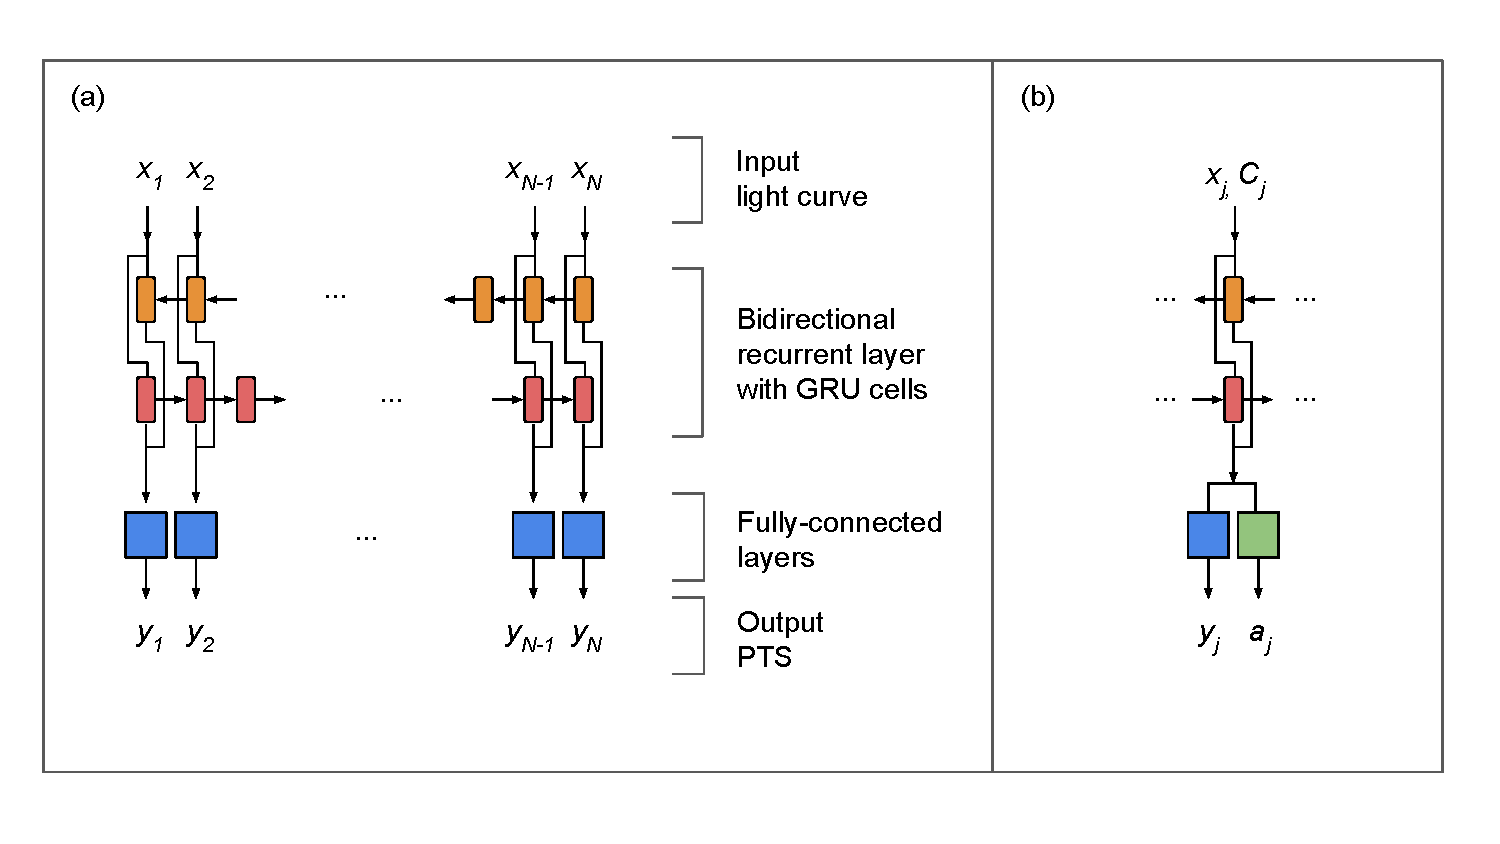
\includegraphics[width=0.7\linewidth]{Methodology/Figures/network_drawing.pdf}
    \caption{(a) The basis RNN which takes as input $x_1,\dots,x_{N}$ and outputs $y_1,\dots,y_{N}$. Colors indicate which blocks share the same weights and arrows indicate the flow of information. The outputs of both components of the bidirectional recurrent layer are concatenated before they are passed to the fully-connected (FC) layers. (b) The network is extended in several ways. First, we may use additional inputs $C_j$, e.g. centroid data, at each time step $j$. Second, we may add an additional network of FC-layers, to obtain an additional outputs $a_j$, e.g. confidence values, or representation vectors. }
    \label{fig:my_label}
\end{figure}

\subsection{Architecture}
\label{sec:architecture}

Since light curves may contain thousands of data points, we avoid the ``vanilla''-RNN, which is known to suffer from vanishing gradients. Other recurrent cells considered were GRU and LSTM. We found GRU to produce better and more stable results than LSTM, which is why we used GRU in our basis RNN design. Both directions in time are relevant for the classification of a data point. For example, both ingress and egress are strong features of a transit signal. This means that at mid-transit, knowing information from both directions could make it easier to classify the data points, compared to only knowing the past. For this reason, we make use of a bidirectional RNN, i.e. bi-GRU.

In order to classify each time step as signal or non-signal, the output of the network should be a single value at each time step. To achieve this, we apply fully connected (FC) layers to the outputs of the recurrent layers, which project the hidden representation at each time step down to a single node. The result is passed through the sigmoid activation function, so the outputs lie between 0 and 1. Between fully connected layers, the ReLU activation function is applied to introduce non-linearities. For most experiments, we used a bi-GRU with a single recurrent layer consisting of 64 hidden nodes, and two fully connected layers, both consisting of 64 nodes. This network was obtained by informal hyperparameter tuning, and comparison against different architectures (see Section \ref{sec:models}).

\subsection{Training}
\label{sec:training}

In a supervised fashion, we train the network to classify data points as signal or non-signal. This requires knowing the ground truth of the data. In our case we use simulated data, so we have access to the ground truth. Alternatively, one could use known (non-)transit signals in real-world light curves as ground-truth, or inject simulated transit signals in real-world light curves. 

Typical light curves, however, contain too many data points to be used for training directly. First of all, the training procedure requires storing the gradients at each time step which would quickly overflow memory. Second of all, the RNN cannot well learn dependencies over thousands of time steps, because even LSTM and GRU have forget and reset gates, so using full-length light curves for training would be unnecessarily inefficient. Therefore we assume that the data used for training consists of light curve segments, obtained by splitting the original light curve in segments of equal length $N$. $N$ should be chosen larger than the typical transit duration ($\sim$6 hours) so sufficient background activity is included in the segments, but small enough to allow for efficient training. This work uses $N=1500$ for the training of the network, which corresponds to 50 hours for a cadence of 2 minutes, unless stated otherwise.


The network is used to model $p(T|X)$, where $T$ represents the targets $\{t_j\}_{j=1}^N$ for each data point $\{x_j\}_{j=1}^N$ in a given light curve segment $X$. We assume the network inputs to be preprocessed such that the flux values $x_j$ can take any value, i.e. $x_j \in \mathbb{R}$. A target $t_j$ is 1 if $x_j$ is part of a transit signal, otherwise it is 0. We assume that the target $t_j$ depends on all flux values through $x_j$, which is dependent on its neighbours $x_{j\pm1}$, which are dependent on their neighbours, and so on. This can be visualized by:

\begin{figure}[H]
\centering
  \tikz{
% nodes
%  \node[obs]
 \node (xa) {$\dots$};%
 \node[obs,right=of xa] (xb) {$x_{j-1}$};%
 \node[obs,right=of xb] (xc) {$x_{j}$};
 \node[obs,right=of xc] (xd) {$x_{j+1}$};
 \node[right=of xd] (xe) {$\dots$};%
 
 \node[latent,below=of xb] (tb) {$t_{j-1}$};
 \node[latent,below=of xc] (tc) {$t_{j}$};
 \node[latent,below=of xd] (td) {$t_{j+1}$};

\edge [-] {xb} {xa, xc};
\edge [-] {xd} {xc, xe};
\edge {xb} {tb};
\edge {xc} {tc};
\edge {xd} {td};
  }
\end{figure}
\noindent Since we observe $X$, the targets become separated in the graphical model. Therefore we model them as independent, given $X$, i.e.:
\begin{equation}
    p(T|X) = p(t_1,\dots,t_N|X) = \prod_{j=1}^N p(t_j|X)
\end{equation}
In other words, we assume that knowing the a target $t_{k}$ at time step $k \neq j$ in addition to the flux values $X$, would not make a difference for the probability of observing $t_j = 1$, compared to only knowing $X$. Therefore, the only information we feed to the network at each time step is $x_j$.

Our network outputs a value $y_j \in (0,1)$ for each $x_j$, using the function $Y = f(X, W)$, where $W$ represents the weights of the network. $Y$ represents the collection of outputs $\{y_j\}_{j=1}^N$. We interpret $y_j$ as the conditional probability $y_j = p(t_j=1|X,W)$, such that $p(t_j=0|X,W)$ is given by $1-y_j$. The conditional distribution of targets at time step $j$ is then given by:
\begin{equation}
    p(t_j|X,W) = y_j^{t_j} (1-y_j)^{1-t_j}
\end{equation}

\noindent Given a set of independent observations $\{T_i\}_{i=1}^M$ for light curve segments $\{X_i\}_{i=1}^M$, we aim to maximize the likelihood $p(T|X,W)$ by updating the weights $W$ of the network. Equivalently, we can maximize the log likelihood, which is given by:
\begin{align}
    \log p(T|X,W) &= \sum_{i=1}^M \log  p(T_i|X_i,W) \\
    &= \sum_{i=1}^M \log \prod_{j=1}^N p(t_{ij}|X_i,W) \\
    &= \sum_{i=1}^M \sum_{j=1}^N \log [ y_{ij}^{t_{ij}} (1-y_{ij})^{1-t_{ij}} ] \\
    &= \sum_{i=1}^M \sum_{j=1}^N t_{ij} \log y_{ij} + (1-t_{ij}) \log(1-y_{ij}),
\end{align}

\noindent where $t_{ij}$ represents the target at time step $j$ in light curve $i$ and $y_{ij} = y(X_i,W)_j$.

To define our loss function, which we aim to minimize, we take the negative of $\log p(T|X,W)$, averaged over the number of samples $M$ and the number of data points per sample $N$, i.e. for a single light curve segment $i$ we have the loss:
\begin{equation}
    \mathcal{L}_{\text{BCE},i} = \frac{1}{N}\sum^{N}_{j=1} l_{ij} + (1 - t_{ij}) \log (1 - y_{ij}),
\end{equation}

\noindent where we used $l_{ij} = t_{ij} \log( y_{ij})$, and the subscript BCE because this is known as the binary cross-entropy loss.
Using this loss function for a batched training with $M$ light curve segments per batch, we get:
\begin{equation}
    \mathcal{L}_{\text{BCE}} = \frac{1}{M} \sum_{i=1}^M \mathcal{L}_{\text{BCE},i}.
\end{equation}



In terms of individual data points, however, we are dealing with a highly unbalanced data set, because there are many more non-signal points than signal points. In order to deal with unbalances, we use a different definition of $l_{ij}$:

\begin{equation}
    l_{ij} = p_t w_{ij} t_{ij} \log( y_{ij} ).
\end{equation}

\todo{references of loss weighting}
Here $p_t$ is the positive weight, which is used to tune the weight of positive samples, i.e. the data points which are part of a transit signal. If $p_t > 1$, then the predictions over signal data points will be given extra weight in the loss function. For a given classification threshold, increasing $p_t$ will increase the recall, but will also lower the precision. In addition to the weight $p_t$, which is the same for all positive samples, we explore the use of transit-specific weighting. It might be that the data set contains more shallow than deep transit signals, in which case we may choose to increase the weight of data points belonging to deep transit signals in the data set, and vice versa. This can be done by letting the weight $w_{ij}$ depend on the depth $\delta_{ij}$ of the transit signal at time step $j$. For example, we can set $w_{ij} = \delta_{ij} / \sigma_{i}$, where $\sigma_i$ is the estimated level of white noise in light curve $i$, so $w_{ij}$ depends on the relative transit depth rather than absolute transit depth. In this case, predictions over data points belonging to a transit signal which is twice as deep as another signal in the same light curve, will get twice the weight in the loss function. In case both $p_t$ and $w_{ij}$ are used, a small adjustment to $p_t$ needs to be made for maintaining consistent results between different choices for $w_{ij}$. The new weight for signal data points during training becomes  $p_t' = p_t \cdot \sum_{ij} t_{ij} / \sum_{ij} w_{ij}$, where for $w_{ij} = t_{ij}$ we have $p_t' = p_t$.

Finally, we found that applying weight decay helped to prevent exploding gradients in the GRU. Simply clipping gradients above a certain value would sometimes fail when gradients jumped to infinity in a single training step, causing the training stop before they could be clipped. Weight decay is used as implemented in PyTorch, i.e. decoupled weight decay from \cite{loshchilov2017decoupled}. A weight decay with tuning parameter $\alpha=\num{5e-5}$ was sufficient in most cases.

